\label{c4:minimizer}
\section{Problem setting}
The minimizer scheme~\citep{roberts05,schleimer03} is a sampling method that selects length-$k$ substrings (i.e., $k$-mers) from a string such that sufficient information about the identity of the sequence is preserved, typically for comparison purpose. It is widely used to reduce memory consumption and run-time in bioinformatics applications such as genome assemblers~\citep{ye12}, read mappers~\citep{jain20,li18minimap2} and $k$-mer counters~\citep{deorowicz15kmc,erbert17gerbil}. 

Our discussion of the minimizer scheme will be grounded in sequences drawn from an arbitrary alphabet $\Sigma$. To begin, let us define some useful notations. Given some parameter $k$, a $(w,k)$-window is defined as a substring of length $w_k=w-k+1$, which contains exactly $w$ overlapping $k$-mers. Let $S \in \Sigma^{L+k-1}$ be sa string containing exactly $L$ overlapping $k$-mers and $L_w\triangleq L-w+1$ overlapping $(w,k)$-windows. Generally, we assume that $w\ll L$ and $k\ll L$, as is typical in most practical settings. We use the notations $\kappa^k_i$ and $\kappa^{w_k}_i$ to respectively denote the $i^{\text{th}}$ $k$-mer and the $i^{\text{th}}$ $(w, k)$-window in $S$. 

Generally, a $k$-mer sampling scheme is a function $\mathcal{X}$ such that $\mathcal{X}(S) \in 2^{[L]}$ returns a set of $k$-mer locations in $S$. The resulting sketch is given by the notation $\mathcal{K}(S; \mathcal{X}) \triangleq \{(\kappa^k_i, i)\}_{i \in \mathcal{X}(S)}$. Note that the sketch report tuples of both $k$-mer and index to distinguish identical $k$-mers sampled from different parts of $S$. We evaluate the performance of such a sampling scheme by computing its density~\citep{marcais17}, which is the fraction of sampled $k$-mers relative to the length of the target sequence:
\begin{eqnarray}
{D}(S; \mathcal{X}) &\triangleq& \frac{\left|\mathcal{K}(S; \mathcal{X}, r)\right|}{L} \ .
\label{c5-eq:density}
\end{eqnarray} 

\noindent The minimizer scheme \cite{schleimer03} is a $k$-mer sampling scheme that makes its sampling decisions based on an arbitrarily constructed total ordering on the $k$-mer set, which is represented by a permutation $\pi$. In particular, we define the minimizer scheme as follows:
\begin{definition}[Minimizer]
\label{c5-def:minimizer}
A minimizer scheme is characterized by a tuple of parameters $(w, k, \pi)$, where $w, k$ are defined above and $\pi$ is a total ordering on the set of all $k$-mers. We define the following selector function, which returns the lowest-ranked $k$-mer in some $(w,k)$-window of $S$: 
\begin{eqnarray}
m(\kappa^{w_k}_v; \pi) &\triangleq&  \underset{i \in [1, w]}{\mathrm{argmin}} \ \sum_{j \in [1,w]} \mathbb{I}(\kappa^k_{v+j-1} <_{\pi} \kappa^k_{v+i-1}) \ ,
\label{c5-eq:minimizer}
\end{eqnarray}
where $\kappa^k_{v+i-1}$ denotes the $i^{\text{th}}$ $k$-mer in the window $\kappa^{w_k}_v$ and $\mathbb{I}(\kappa <_{\pi} \kappa')$ denotes the event that $\kappa$ precedes $\kappa'$ in $\pi$ for some $\kappa,\kappa' \in \Sigma^k$. The minimizer sampling function is then given by:
\begin{eqnarray}
\mathcal{M}(S;w,k,\pi) \triangleq \{i + m(\kappa^{w_k}_i;\pi)\}_{i\in[L_w]} \ ,
\label{eq:mnzsketch}
\end{eqnarray}
which iteratively applies $m$ on every window in $S$.
\end{definition}
 A low-density minimizer scheme achieves three desiderata: (1)~the sketch is compact and will offer significant cost saving to downstream applications; (2)~every $(w,k)$-window in $S$ overlaps at least one $k$-mer in the sketch; and (3)~identical windows are represented by the same $k$-mer due to the deterministic sampling protocol. These properties give rise the minimizer sketch design (MSD) problem below.
\begin{definition}[Low Density Minimizer Sketch Design]
\label{c5-def:minimizerproblem}
Let $S$ be a string defined as above. Suppose $w$, $k$ and $r$ are given as application-specific parameters, the minimizer selection problem is defined as:
\begin{eqnarray} 
 \pi_\ast &=& \underset{\pi \in \Pi(\Sigma^k)} {\mathrm{argmin}} \ \mathcal{D}(S; \mathcal{M}(\pi)) \ ,
\label{c5-eq:obj}
\end{eqnarray}
where $\Pi(\Sigma^k)$ denotes the set of all $k$-mer permutations in $\Sigma^k$ and we write $\mathcal{M}(\pi)$ to clearly show the dependency of $\mathcal{M}$ on the $k$-mer ordering $\pi$, which is being optimized.
\end{definition} 

\noindent Another recently suggested sketching desiderata~\citep{edgar2021syncmers} is that two substrings differing only by a few mutations are likely represented by the same $k$-mer in the sketch. \citet{edgar2021syncmers}~argues that the density metric above is not sufficient to capture this, and hence proposes an alternative metric called \textit{conservation}:
\begin{eqnarray}
{C}(S; \mathcal{X}) &\triangleq& \mathbb{E}_{S'}\left[\frac{\left|\mathcal{K}(S; \mathcal{X}) \cap \mathcal{K}(S'; \mathcal{X})\right|}{L}\right]\ ,
\label{c5-eq:cons}
\end{eqnarray} 
which measures the expected fraction of selected $k$-mers (relative to the length of $S$) that are preserved under random mutation (i.e., higher is better). Here, $S'$ is a copy of $S$ with randomly substituted characters and the conservation metric is expected over the distribution of $S'$. To obtain high conservation sketches \citet{edgar2021syncmers} also proposes another sketching method called \emph{syncmers}.
\begin{definition}[Syncmer]
\label{c5-def:syncmer}
A syncmer scheme is defined by a tuple of parameters $(k, s, t, \pi)$, where $k$ similarly denotes the substring length to be sampled (i.e., $k$-mers) and $s, t \in [1,k]$. Here, $\pi$ is a permutation of all $s$-mers in $\Sigma^s$. Similar to Definition~\ref{c5-def:minimizer}, we also define a selector function, which now returns the lowest-ranked $s$-mer in some $k$-mer of $S$: 
\begin{eqnarray}
m(\kappa^k_v; \pi) &\triangleq& \underset{i \in [1,k]}{\argmin} \sum_{j\in[1,k_s]} \mathbb{I}(\kappa^s_{v+j-1} <_{\pi} \kappa^s_{v+i-1}) \ ,
\end{eqnarray}
where $k_s \triangleq k-s+1$ denotes the number of overlapping $s$-mer in a $k$-mer. The syncmer sampling function is then specified by iteratively sampling any $k$-mer such that its lowest-ranked $s$-mer is at the $t^{\text{th}}$ position:
\begin{eqnarray}
\mathcal{O}_t(S; k, s, \pi) \triangleq \{i \mid m(\kappa^k_i; \pi) = t\}_{i\in [L]} \ .
\end{eqnarray}
We specially choose to write $t$ as a subscript since syncmer schemes with similar $k, s, \pi$ initialization and different offset $t$ are theoretically related, as shown below in the technical approach.
\end{definition}
Although there has been no explicit sketch design method developed for syncmers (i.e., optimizing the $s$-mer permutation $\pi$), \citet{edgar2021syncmers}~and \citet{shaw2021theory}~have empirically observed that the syncmer method is capable of simultaneously achieving both lower density and higher conservation than the minimizer method when both use a random ordering. Nonetheless, no formal relationship has been established between the two methods due to the lack of a convention to compare them.

This chapter explores a new approach for solving the minimizer sketch design problem via a differentiable reformulation of the permutation learning task in Definition~\ref{c5-def:minimizer}, called \textsc{DeepMinimizer}. We then derive the first theoretical relationship between the density and conservation metrics; as well as between the minimizer and syncmer methods. This new insight allows us to (1)~unify minimizers and syncmers under a generalized notion of sequence sketching called \textit{masked minimizer}; and (2)~extend our \textsc{DeepMinimizer} framework to automate \textit{masked minimizer} sketch design.

\section{Related work}
\subsection{UHS-based methods} Most existing minimizer selection schemes with performance guarantees over random sequences are based on the theory of universal hitting sets (UHS)~\citep{marcais18,orenstein17}. Particularly, a $(w,k)$-UHS is defined as a set of $k$-mers such that every window of length $w$ (from any possible sequence) contains at least one of its elements. Every UHS subsequently defines a family of corresponding minimizer schemes whose expected densities on random sequences can be upper-bounded in terms of the UHS size~\citep{marcais17}. As such, to obtain minimizers with provably low density, it suffices to construct small UHS, which is the common objective of many existing approaches~\citep{marcais17,ekim20pasha,zheng20miniception}. These methods, however, rely on the unrealistic assumption that the target sequences follow a uniform distribution~\citep{zhang07}. As such, there tends to be little correspondence between the provable upper-bound on expected density and the actual density measured on a target sequence. 

\subsection{Heuristic methods} Several minimizer construction schemes rank $k$-mers based on their frequencies in the target sequence~\citep{chikhi16,jain20b}, such that infrequent $k$-mers are more likely to be chosen as minimizers. These constructions nonetheless rely on the assumption that infrequent $k$-mers are spread apart and ideally correspond to a sparse sampling. Another greedy approach is to sequentially remove k-mers from an arbitrarily constructed UHS, as long as the resulting set still hits every $w$-long window on the target sequence~\citep{deblasio19}. Though this helps to fine-tune a given UHS with respect to the sequence of interest, there is no guarantee that such an initial set will yield the optimal solution after pruning.

\subsection{Polar set construction} Recently, a novel class of minimizer constructions was proposed based on polar sets of $k$-mers, whose elements are sufficiently far apart on the target sequence~\citep{zheng21}. The sketch size induced by such a polar set is shown to be tightly bounded with respect to its cardinality. This reveals an alternate route to low-density minimizer schemes through searching for the minimal polar set. Unfortunately, this proxy objective is NP-hard and currently approximated by a greedy construction~\citep{zheng21}, which can be sub-optimal in practice.

\section{Differentiable reformulation of the MSD problem}
\subsection{Motivation}
The technical challenges of the MSD problem described above arise due to two factors. First, the search space is factorially large in terms of $k$. Exhaustively searching this domain of $k$-mer permutations would suffice for very small $k$, but will quickly become intractable for larger values of $k$ that are typically used in many practical applications. Second, the density minimizing objective is discrete, hence difficult to be optimized via standard techniques. 

All existing MSD frameworks approach this optimization problem by approximating its permutation search space (i.e., space of total $k$-mer orderings) with the space of partial $k$-mer orderings that satisfy certain surrogate properties. For example,~\citet{marcais17,marcais18,ekim20pasha,zheng20miniception} adopt the universal hitting set (UHS) approximation which imposes that all $k$-mers in a selected UHS will be ranked with lower priorities than those outside. The polar set (PS) approximation proposed by~\citet{zheng21} is similar in spirit, but uses a different set of surrogate properties to construct these partial orderings.

The main advantage of these strategies is that they reduce the permutation learning objective in Definition~\ref{c5-def:minimizerproblem} to finding the most compact construction of such surrogate sets, which is relatively simpler to achieve. However, these approximations either rely on unrealistic assumptions about the target sequence, such as its characters are uniformly distributed (e.g., UHS-based methods~\cite{marcais17,marcais18,ekim20pasha,zheng20miniception}); or remain a challenging discrete objective that can only be solved via greedy heuristics (e.g., the PS method~\cite{zheng21}). Furthermore, both of these approximation schemes can be viewed as domain restriction techniques where the sets of active candidates are confined to UHS/PS-induced permutations. Nonetheless, there is no guarantee that these active sets would necessarily contain the optimal solution.

To overcome these challenges, we instead propose a re-parameterization of the original permutation learning problem, which implicitly casts the $k$-mer permutation $\pi$ as a function $f_\pi: \Sigma^k \rightarrow [0,1]$ that assign continuous scores to $k$-mers in $\Sigma^k$. Every \emph{valid} candidate function must be a consistent scoring scheme (i.e., a $k$-mer will get the same score regardless of its position and local neighborhood in the target sequence), such that a permutation can always be recovered via sorting the scores. Modelling the space of such valid functions with a deep neural network, we subsequently propose to cast the MSD problem as a deep learning optimization task with respect to the density objective in Definition~\ref{c5-def:minimizerproblem}. We further note that, unlike existing approximations, the candidate set encoded by our re-parameterization can theoretically approach the unrestricted permutation domain $\Pi(\Sigma^k)$ given a sufficiently expressive network architecture.

\begin{figure}[ht]
\centering
\begin{tabular}{c}
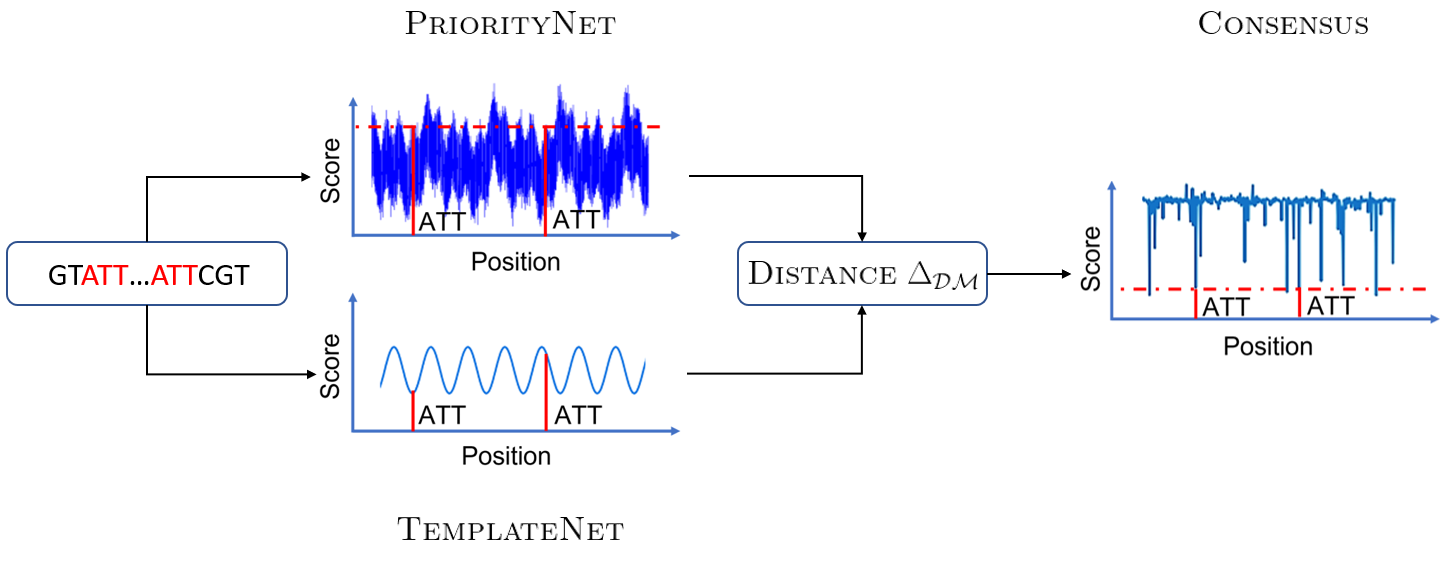
\includegraphics[width=0.95\columnwidth]{minimizer_plots/Schematic.png} 
\end{tabular}
\caption{The \textsc{DeepMinimizer} framework is comprised of two continuous $k$-mer scoring schemes that correspond to different aspects of a low-density minimizer: \textsc{PriorityNet} assigns scores to $k$-mers in the target sequence such that a total ordering can be recovered via simple sorting; whereas \textsc{TemplateNet} relaxes this consistency constraint to achieve a low-density sketch. Minimizing the distance between their outputs is expected to yield a consensus solution that simultaneously exhibits both properties.}
\label{c5-fig:prioritynet}
\end{figure}
Nonetheless, standard backpropagation methods~\citep{kingma14adam} cannot be directly applied to optimize the density metric, which is discrete and does not have an analytic gradient with respect to the network parameters. To address this challenge, we further adopt a similar approach to the proposed KS framework in Chapter~\ref{c3:kernel}, which hierarchically approximates the search task with multiple sub-tasks that can each be solved more efficiently. In the MSD context, these sub-tasks manifest as a pair of complementary neural networks called \textsc{PriorityNet} and \textsc{TemplateNet}. In particular, the \textsc{PriorityNet} component is parameterized such that it always outputs consistent scoring and is tasked to encode the candidate function space of the minimizer scheme. On the other hand, the \textsc{TemplateNet} component relaxes this consistency constraint in exchange for the ability to encode desirable score assignments (but potentially unmeaningful since it might not be possible to recover a proper minimizer scheme). While the KS framework in Chapter~\ref{c3:kernel} adopts a bi-level optimization approach to alternately solve its sub-tasks (i.e., generative trajectory selection and early stopping policy), both components in this MSD scenario can be simultaneously learned via minimizing the divergence between their outputs, hence resulting in the first differentiable relaxation for the MSD problem. A high-level schematic of our approach is shown in Fig.~\ref{c5-fig:prioritynet}. Last, we propose to demonstrate that our method, titled \textsc{DeepMinimizer} is highly-efficient and capable of finding minimizer schemes that yield significantly more compact sketches on multiple human genome benchmarks. The remainder of this chapter will now provide a summary of our technical approach, which will be presented in details in Appendix~\ref{app:maskmnz} along with our empirical findings.

\subsection{Technical Approach}
Using the notion of the scoring function $f_\pi$, the selector function in Definition~\ref{c5-def:minimizer} can be written as:
\begin{eqnarray}
m(\kappa^{w_k}_v; \alpha) &\triangleq& \underset{i \in [1,w]}{\argmin} \ f_\pi\left(\kappa^k_{v+i-1}; \alpha\right) \ ,
\label{eq:mnzselector}
\end{eqnarray}
where $f: \Sigma^{k} \rightarrow [0, 1]$ is parameterized by a convolutional neural network with weight $\alpha$. The architecture of this network (as discussed in Appendix~\ref{app:maskmnz}) guarantees that $f$ is a valid scoring function (i.e., we can always recover a total ordering over all $k$-mers), that is, for all pairs of indices $i, j \in [L]$, we have:
\begin{eqnarray}
\kappa^k_i = \kappa^k_j &\implies& f(\kappa^k_i) = f(\kappa^k_j) \ .
\end{eqnarray}

\noindent For clarity, we will write the density metric as $\mathcal{D}(S; \mathcal{M}(\alpha))$ to clearly establish the change in parameterization. As discussed in the previous section, $f$ cannot be efficiently optimized with gradient back-propagation methods since the derivative $\frac{\partial\mathcal{D}(S; \mathcal{M}(\alpha))}{\partial\alpha}$ does not exist. To work around this, we introduce a proxy optimization objective that approximates $\mathcal{D}(S; \mathcal{M}(\alpha))$ via coupling $f$ with a positional scoring function $g: [L] \rightarrow [0,1]$ parameterized by weight $\beta$. Unlike $f$, which assigns $k$-mers scores based on their contents, $g$ assigns $k$-mers scores based on their positions in $S$ and is likely not a valid scoring function, i.e., $\kappa^k_i = \kappa^k_j \centernot\implies g(i) = g(j)$. Nonetheless, the context-free function $g$ can be used to generate a $k$-mer sketch by adapting Eq.~\ref{eq:mnzsketch} as:
\begin{eqnarray}
\mathcal{T}(S; \beta) \triangleq \left\{i + \underset{j\in[1,w]}{\argmin} \ g(i+j-1; \beta)\right\}_{i \in [L_w]} \ .
\end{eqnarray}
The \emph{template} $k$-mer sampling scheme $\mathcal{T}$ does not have the same desiderata as a minimizer sketch, but we can guarantee that the sketch density is equal to that of an optimal minimizer sketch through carefully constructing $g$, i.e., $\mathcal{D}(S; \mathcal{T}(\beta)) \simeq 1/w$. As $\mathcal{K}(S; \mathcal{M}(\alpha), r)$ corresponds exactly to a minimizer sketch and $\mathcal{K}(S; \mathcal{T}(\beta), r)$ approximates the low-density objective, this reveals an interesting factorization of the search task, and therefore an alternative pathway to the optimal solution through finding a \emph{consensus solution} between the two sketches. Formally, let $\mathbf{f}(S,\alpha) = [f(\kappa^k_i;\alpha)]_{i\in[L]}$ and $\mathbf{g}(\beta) = [g(i)]_{i\in[L]}$ respectively denote the concatenated score vectors that $f$ and $g$ assign to $k$-mers in $S$, we then characterize this consensus solution as a joint instantiation of $\alpha$ and $\beta$ such that some distance metric $\Delta$ between $\mathbf{f}(S,\alpha)$ and $\mathbf{g}(\beta)$ is minimized. Explicitly, this results in the following optimization objective:
\begin{eqnarray}
(\alpha_\ast,\beta_\ast) &\triangleq& \underset{\alpha, \beta}{\argmin} \ \Delta\left(\mathbf{f}(S,\alpha),\mathbf{g}(\beta)\right) \ ,
\end{eqnarray}
which is fully differentiable with respect to weights $\alpha$ and $\beta$. We fully describe our approach, including the parameterizations of $f$, $g$ and the distance metric $\Delta$ in Appendix~\ref{app:maskmnz}.
\section{Unifying minimizer and syncmer sketching methods}
\subsection{Motivation}
Although both minimizers and syncmers employ the same concept of sampling based on a substring total ordering, a minimizer scheme that uses an $s$-mer ordering will directly report $s$-mers in its sketch, whereas a syncmer scheme parameterized by the same ordering will typically report longer $k$-mers. Due to this mismatch in representation, existing work~\cite{edgar2021syncmers,shaw2021theory} all chose to compare schemes that report similar-sized substrings regardless of their ordering choices, which results in an asymmetry of information among their sketches and prevents the derivation of any meaningful correspondence between minimizers and syncmers. 

This shortcoming motivates a revision of the comparability notion for sketching methods. In particular, we advocate comparing schemes that use the same substring ordering to make sampling decisions. This new mode of comparison allows us to explicitly bound the density and conservation gaps between minimizers and syncmers. Building on this theoretical result, we further propose a novel concept of masked minimizers that unify both minimizers and syncmers. The masked minimizer scheme combines the standard minimizer sampling with an additional sub-sampling step, which applies a binary mask filter to the $k$-mer selection at every window. Interestingly, varying this mask parameter induces a spectrum of comparable schemes and reveals a methodical approach to derive comparable sketching schemes. Last, we propose an extension of the \textsc{DeepMinimizer} method to optimize the masked minimizer scheme with respect to a novel sketching metric called the \emph{generalized sketch score} (GSS), which combines both  density and conservation metrics, resulting in the first formal protocol to compare sequence sketching methods.
\subsection{Technical approach}
To explicitly reason about the difference in terms of sketch representation between minimizers and syncmers, we introduce the notion of a reporting function $r$, which maps the sampled locations in $\mathcal{X}(S)$ to tuples of substrings and locations. That is, the reported sketch is now constructed as $\mathcal{K}(S; \mathcal{X}, r) \triangleq \{r(i)\}_{i \in \mathcal{X}(S)}$. Setting $r(i) = (\kappa^k_i, i)$ recovers both Definition~\ref{c5-def:minimizer} of a minimizer scheme with parameters $w, k$ and $\pi_m \in \Pi(\Sigma^k)$; and Definition~\ref{c5-def:syncmer} of a syncmer scheme with parameters $k, s, t$ and $\pi_o \in \Pi(\Sigma^s)$. Since these methods both report $k$-mers, they are traditionally deemed comparable.

This mode of comparison, however, does not facilitate a theoretical analysis of their performance differences (i.e., in terms of density and conservation metrics), as different information bases are used to enact the sampling decisions of a length-$k$ minimizer and syncmer. In particular, $(w, k)$-minimizer schemes use total $k$-mer orderings to perform sampling, whereas $(k, s, t)$-syncmer schemes use total $s$-mer orderings, with $s \leq k$. We note that these bases are only comparable when setting $s=k$, but doing so results in trivial syncmer schemes that selects every $k$-mer in $S$. 

To correct this asymmetry of information, we propose the notion of $\pi$-comparable minimizers and syncmers, which are schemes that employ the same ordering $\pi$. For example, the $(w, k, \pi)$-minimizer and the $(w_k, k, t, \pi)$-syncmer schemes with $w_k\triangleq w+k-1$ and any $t \leq w$, which respectively report $k$-mers and $w_k$-mers, are $\pi$-comparable. To normalize the difference in representation, we replace the default $w_k$-mer reporting function $r(i)=(\kappa^{w_k}_i, i)$ of the above syncmer scheme with the $k$-syncmer reporting function $r'(i)=(\kappa^k_{i+t}, i+t)$. As both reporting functions are one-to-one mappings of the selected locations, this substitution results in a semantically equivalent \textit{shifted} syncmer scheme.

This translation of the reporting function aligns our proposed comparison with the traditional perspective of comparability and presents an invariant substring ranking behavior among the compared schemes, which subsequently allows us to derive explicit bounds on their density and conservation gaps. In particular, we prove that the density and conservation of any syncmer on a specific sequence $S$ are respectively upper-bounded and almost surely upper-bounded by that of its $\pi$-comparable minimizer, thus establishing the first theoretical correspondence between $\pi$-comparable schemes. Our theoretical result is summarized in Theorem~\ref{c5-theo:1}, whose detailed proof is given Appendix~\ref{app:maskmnz}.
\begin{theorem}[$\pi$-comparability defines a correspondence between minimizers and syncmers] For \linebreak every syncmer scheme  $(\mathcal{O}_t, r')$, there exists a comparable minimizer scheme $\mathcal{M}$ whose reporting function $r$ is translated from $r'$ with an offset $t$, such that the following bounds hold for every $S \in \Sigma^{L+k-1}$: 
\begin{eqnarray}
D(S; \mathcal{O}_t,r') \ \leq 
 \ D(S; \mathcal{M},r) \qquad \text{and} \qquad  C(S; \mathcal{O}_t,r') \ \leq \ C(S; \mathcal{M},r) + \frac{t}{L} \ .
\end{eqnarray}
\label{c5-theo:1}
\end{theorem}
We then further show that any syncmer scheme can be recovered given a $\pi$-comparable minimizer $\mathcal{M}$ via sub-sampling the set of locations selected by $\mathcal{M}$. We write this sub-sampling rule as follows:
\begin{eqnarray}
\mathcal{O}_t(S) &=& \left\{
i - t \mid \left\|    \overrightarrow{m}(\kappa^{w_k}_{i-t};\pi) \otimes \mathbf{e}_t
\right\|_1 > 0
\right\}_{i \in \mathcal{M}(S)} \ ,
\end{eqnarray}
where $\overrightarrow{m}(\kappa^{w_k};\pi) \triangleq [\mathbb{I}(j=m(\kappa^{w_k}; \pi))]_{j\in[w]}$ is the one-hot representation of the $k$-mer selection result at some arbitrary window $\kappa^{w_k}$ using the selector function $m$; $\mathbf{e}_t$ denotes the one-hot vector with a non-zero entry on the $t^{\text{th}}$ row; and $\otimes$ denotes the pointwise multiplication operator. The sub-sampling condition above checks if any position remains selected after filtering with $\mathbf{e}_t$ (in which case, it must be the $t^{\text{th}}$ position). Interestingly, this sub-sampling rule can be generalized by replacing $\mathbf{e}_t$ with any arbitrary $w$-dimensional binary mask $\nu \in \{0,1\}^w$. For example, setting $\nu=\mathbf{1}_w$ trivially recovers the standard minimizer scheme (without applying the offset $t$). Given a set of minimizer-sampled locations $\mathcal{M}(S)$,  varying $\nu$ yields a total of $2^w$ $\pi$-comparable schemes, leading to a unifying method called \textit{masked minimizers}. 
\begin{definition}[Masked minimizers] 
The sampling function of a masked minimizer scheme is characterized by a tuple of parameters $(w, k, \pi, \nu)$, where $w,k,\pi$ correspond to standard minimizer parameters, and $\nu\in\{0,1\}^w$ is a $w$-dimensional binary vector. The masked minimizer sampling function is given by:
\begin{eqnarray}
\mathcal{V}(S; w,k,\pi,\nu) \ \triangleq \ \{i + m(\kappa^{w_k}_i; \pi) \mid \zeta(\kappa^{w_k}_i, \nu)\}_{i\in[L_w]} \ ,
\end{eqnarray}
where $\zeta(\kappa^{w_k}_i, \nu) \triangleq \|\overrightarrow{m}_\pi(\kappa^{w_k}_i) \otimes \nu]\|_1 > 0$ denotes the event that the selection at the $i^{\text{th}}$ window remains sampled after applying the sub-sampling mask.
\end{definition}

\noindent We also show that improving density places an upper-bound on how much conservation can be improved and vice versa, which implies that neither objective should be considered independently of one another. To account for this trade-off, we propose a new metric called the \emph{generalized sketch score} (GSS):
\begin{eqnarray}
G(S; \mathcal{X}, r, w) &\triangleq& \frac{C(S;\mathcal{X},r)}{D(S;\mathcal{X},r)} \cdot \frac{1}{L_w} \sum_{i=1}^{L_w} V_i(S; \mathcal{X}, w) \ ,
\end{eqnarray}
where $V_i(S;\mathcal{X}, w) \triangleq 1 - \prod_{j=i}^{i+w-1} \mathbb{I}(j \not\in \mathcal{X}(S))$ is the indicator variable of the event that the window $\kappa^{w_k}_i$ overlaps at least one sampled location in $\mathcal{X}(S)$. The GSS metric seeks to capture the trade-off between density and conservation via the ratio $C(S;\mathcal{X}, r)/D(S;\mathcal{X},r)$ and further prevents possible trivial exploitation with the \emph{coverage} term $\sum_{i=1}^{L_w} V_i(S; \mathcal{X}, w)$. We provide the full explanation regarding the benefits of this metric in Appendix~\ref{app:maskmnz}.

Finally, we propose an extension of the \textsc{DeepMinimizer} method to optimize a masked minimizer scheme with respect to the GSS metric. In particular, our new objective is given as a bilvel optimization:
\begin{eqnarray}
(\alpha_\ast,\beta_\ast) &\triangleq& \underset{\alpha, \beta}{\argmin} \ \Delta\left(\mathbf{f}(S,\alpha),\mathbf{g}(\beta)\right) + \sum_{i=1}^n \Delta\left(\mathbf{f}(S_i,\alpha),\mathbf{f}(S, \alpha)\right) \ , \nonumber \\
\quad \nu_\ast &\triangleq& \underset{\nu}{\argmin} \ G(S; \mathcal{V}(\alpha_\ast), r, w) \ ,
\end{eqnarray}
where $S_1, S_2, \dots, S_n$ denote $n$ randomly sampled mutations of $S$; $\Delta$, $\mathbf{f}$ and $\mathbf{g}$ are previously defined in the technical exposition of the \textsc{DeepMinimizer} method. The first optimization adds an extra term to the \textsc{DeepMinimizer} loss, which measures the expected distance between each priority vector $\mathbf{f}(S_i,\alpha)$ for mutated sequence $S_i$ and the original template vector $\mathbf{f}(S,\alpha)$. As the priority vector is a surrogate for the actual discrete $k$-mer selection, minimizing this term will likely improve the stability of selection (i.e., conservation) when the sequence is subjected to random mutations. The second optimization, on the other hand, is written as a greedy search to find the optimal mask given an ordering induced by the parameter $\alpha_\ast$ obtained from the first optimization. We detail our approach in Appendix~\ref{app:maskmnz}.

\section{Results}
To demonstrate the performance of \textsc{DeepMinimizer}, we compare our method with the following benchmarks: (a)~A random minimizer (the total ordering $\pi$ is uniformly sampled); (b) \textsc{Miniception}~\cite{zheng20miniception}; (c) \textsc{PASHA}~\cite{ekim20pasha}; and (d) \textsc{PolarSet}~\cite{zheng21}. We use the following sequence benchmarks to conduct our empirical study: (a)~human chromosome 1 (\textsc{Chr1}); (b) ~human chromosome X (\textsc{ChrX}); (c) ~the centromere region of chromosome X (\textsc{ChrXC}); (d) ~the full human genome (\textsc{Hg38}). The full details of these sequences are given in Appendix~\ref{app:maskmnz}.

We first compare the minimizer sketch before and after training with \textsc{DeepMinimizer} to demonstrate that \textsc{DeepMinimizer} results in a sparse selection of $k$-mers in the target sequence. Across many settings of $w$ and $k$, we show that \textsc{DeepMinimizer} consistently converges to a low-density sketch, which shows that our objective function correlates well with the density metric. We also conduct ablation studies to study the effect of different template functions and distance functions, which justify our empirical choices. 

To demonstrate the effectiveness of our masked minimizers unification approach and justify our theoretical insight, we further conduct extra experiments to answer the following questions:
(1)~Are density and conservation adversarially related? (2)~How do $\pi$-comparable schemes perform relative to one another under the proposed metric GSS? (3)~Can mask optimization improve the overall performance of both minimizer and syncmer? Through these demonstrations, we confirm our theoretical understanding of various sketching metrics and the relationship among $\pi$-comparable schemes, as well as demonstrate the efficiency of our proposed optimization method.

Our experiments show that density and conservation metrics indeed have an adversarial relationship. In addition, our masked minimizer training method is highly effective in optimizing their trade-off. We demonstrate this effectiveness in many settings of $w, k$ and binary mask $\nu$. Last, we also demonstrate that selecting an optimal mask can have significant effect on the GSS of sketching methods. We test this on sequence patterns that are known to be difficult for standard minimizer methods and show that our approach are capable of finding masks that improve the performance.

We give the full details of our empirical study to Appendix~\ref{app:maskmnz}. Our work on the \textsc{DeepMinimizer} method has been published at the International Conference on Research in Computational Molecular Biology (RECOMB 2022). Our work on the unifying masked minimizer approach is currently under review for RECOMB 2023.